\documentclass[a4paper,11pt]{article}

\usepackage[T1]{fontenc} 
\usepackage[latin1]{inputenc}

\usepackage{listings} \lstset{language=c, showstringspaces=false}

\usepackage{graphicx}


\newcommand{\nnsection}[1]{
\section*{#1} \addcontentsline{toc}{section}{#1} }

\begin{document}

\begin{center} \vspace{20pt} \textbf{\large Page frame reclaiming algorithms}\\
\vspace{10pt} \textbf{Johan Montelius}\\ \vspace{10pt} \textbf{VT2016}
\end{center}

\nnsection{Introduction}

In this assignment you will explore some of the page frame reclaiming
algorithms that you have read about.

\section{Pick one by random}

To set a standard and to see if we actually do something useful we
first implement the algorithm where we select a frame by random. If we
later experiment with very complicated algorithms we hope that they
behave better than the random, or why would we else bother to implement
something complicated.

Create a file {\tt random.c} and open up your favorite editor. Don't
use an IDE that hide all the complicated things, use a regular text
editor and do the compilation by hand from a command shell. 

\subsection{a random sequence}

The first thing we shall do is to generate a random sequence of page
identifiers. This sequence is the sequence of page references that we
are going to use in our benchmark of the algorithm. We could have
generated these references on the fly but we need them when we
implement the optimal strategy so we might as well do it now. 

Below is you first go at the {\tt random.c} program. It will only
write out a sequence of random numbers but it's only a start.  Compile
the code and do a test run to see that it works.


\begin{lstlisting}
#include <stdio.h>
#include <stdlib.h>
#include <math.h>
#include <assert.h>

void init(int *sequence, int refs, int pages)  {
  for(int i = 0; i<refs; i++) {
    sequence[i] = rand()  %pages;
  }
}

int main(int argc, char *argv[]) {

  /* could be command line arguments */
  int refs = 10;
  int pages = 100;
  
  int *sequence = (int*)malloc(refs*sizeof(int));

  init(sequence, refs, pages);

  /* a small experiment to show that it works */
  for(int i = 1; i < refs; i++) {
    printf(", %d", sequence[i]);
  }
  printf("\n");  

  return 0;
}
\end{lstlisting}

So we have a random sequence of references but we need to make things
a bit more interesting. The more advanced algorithms are based on the
fact that page references will probably not be completely
randomized. They make use of the fact that some pages are referenced
more often compared to other pages etc. To make the sequence look more
like a real life sequence we change the initialization so that it will
produce a sequence where 20\% of the pages are referenced 80\% of the
time (spatial locality). 


\begin{lstlisting}
/* 20% of the pages will have 80% of the references */  
#define HIGH 20
#define FREQ 80

void init(int *sequence, int refs, int pages)  {

  int high = (int)(pages*((float)HIGH/100));

  for(int i = 0; i<refs; i++) {
    if(rand()%100 < FREQ) {
      /* the frequently case */
      sequence[i] = rand()%high;        
    } else {
      /* the less frequently case */
      sequence[i] = high + rand()%(pages - high);
    }
  }
}
\end{lstlisting}

Note that this is a very crude way of approximating a sequence of page
references. There is for example no {\em temporal locality} that would
make it more likely that we reference pages that we have recently
referenced. To capture this we would have to include a memory in the
generator so that it had a preference for say the last ten pages
rather than jumping to a random page. 

The model we have will do for our simple experiment but to do a better
evaluation one would need a better approximation and of course actual
data from real executions. 

\subsection{keep track of the pages}

In our experiments we will not swap pages in our out but simply keep
track of how many time we would have to do it if we actually used the
algorithms in a real system. We can therefore keep things quite simple
and only track if a page is allocated or not. We will keep a {\em page
  table} with one entry per page and each entry, a {\em page table
  entry}, will tell us if a page is in memory or not (the {\em
  presence bit}).

\begin{lstlisting}
typedef struct pte {
  int present;
} pte;
\end{lstlisting}

In the main procedure we allocate memory for the page table.  If we
know that we always will use a page table of size $100$ we can
 allocated it on the stack using the following construct (with PAGES defined as a macro).

\begin{lstlisting}
  pte table[PAGES];
\end{lstlisting}

If we rather have the number of pages being given at run-time we need
to allocate the structure on the {\em heap} using a call to {\tt
  malloc()}.  The same 

\begin{lstlisting}
  pte *table = (pte *)malloc(pages*sizeof(pte));
\end{lstlisting}


\subsection{the simulation}

Now we're ready to do the simulation and we will simulate what would
happen in a system with a given set of frames. As the number of frames
increase we will have room for more of the pages and when we have as
many frames as we have pages there will be no swapping at all.

This is the structure of the benchmark, we compute a increment, the
number of pages divided by the number of data points, and then run the
simulation for a growing number of frames. Keep the output as shown,
we will later process the data and produce a nice graph. The procedure
{\tt clear\_page\_table(int *page\_table, int pages)} should run through
the page table and set the present bits to zero. Complete the code
with SAMPLES as a defined macro set to $20$.

\begin{lstlisting}
printf("# This is a benchmark of random replacement\n");
printf("# %d page references\n", refs);
printf("# %d pages \n", pages);
printf("#\n#\n#frames\tratio\n");
  
/*  frames is the size of the memory in frames */
int frames;

int incr = pages/SAMPLES;
  
for(frames = incr; frames <= pages; frames += incr) {

  /* clear page tables entries */
  clear_page_table(table, pages);

  int hits =  simulate(sequence, table, refs, frames, pages);

  float ratio = (float)hits/refs;

  printf("%d\t%.2f\n", frames, ratio);
}
\end{lstlisting}
 
The {\tt clear\_page\_table()} is easily defined as below.

\begin{lstlisting}
void clear_page_table(pte *page_table, int pages) {
    for(int i=0; i < pages; i++) {
      page_table[i].present = 0;
    }
}
\end{lstlisting}


In the heart of the simulator we read the references one by one to
determine if it would have given us a hit in the memory or a page
fault. If we have a hit we're happy, but if not we have to do some
more work. If we still have free frames we simply mark the page as being in
memory but if the number of allocated pages is equal to the available
number of frames we need to evict a page. 

\begin{lstlisting}
int simulate(int *seq, pte *table, int refs, int frms, int pgs) {

  int hits = 0;
  int allocated = 0;
    
  int i;
	
  for(i = 0; i < refs; i++) {
    int next = seq[i];
    pte *entry = &table[next];

    if(entry->present == 1) {
      hits++;
    } else {
      if(allocated < frms) {
	allocated++;
	entry->present = 1;
      } else {
	pte *evict;
	do {
	  int rnd = rand()%pgs;
	  evict = &table[rnd];
	} while(evict->present != 1);

	evict->present = 0;
	entry->present = 1;
      }
    }
  }
  return hits;
}
\end{lstlisting}

In this simulation we will select a page by random. We will not be very
efficient in this process (why?) but for our purposes its fine. We
simply generate a random page number and check if it's in memory. When
we find a page we simply mark it as swapped and mark the new page as
in memory.

\subsection{generating a graph}

If you have the program up and running you should be able to able to
generate a sequence of data points. This is all fine but we would like
to generate a nice graph on the fly.

\begin{verbatim}
# This is a benchmark of random replacement policy
# 100000 page references
# 100 pages 
#
#
#frames	ratio
5	0.13
10	0.28
15	0.41
 :
\end{verbatim}

The first thing we do is to write the output to a file. We could have
written our program in a way where it opens and writes the data to the
file but a simpler way is to use the shell to do it for us. Try the
following in your shell:

\begin{verbatim}
$ gcc random.c  -o random
$ ./random > random.dat
$ more random.dat 
\end{verbatim}

So now we have a file called {\tt random.dat} with the data that we
want to plot. Now in a shell run the program {\tt gnuplot}, if it's
not installed it should be a 2 min job to install it. If gnuplot
starts, try the following:

\begin{verbatim}
gnuplot> plot "random.dat" u 1:2
\end{verbatim}

If everything works you should see a window with a nice graph of the
data points. You have just told gnuplot to plot the data in the file
{\tt random.dat} using the columns 1 and 2. Gnuplot will ignore all
lines starting with a {\tt \#} so this is why we generated the output like we did.

You can explore gnuplot using the command line but after a while you
want to write a script that generates the plot that you want to
have. Save the following in a file called {\tt random.p}.

\begin{verbatim}
# Gnuplot script for plotting data in file "random.dat"
set terminal png
set output "random.png"

set title "Page replacement using random policy"

set key right center
    
set xlabel "frms in memory"
set ylabel "hit ratio"    

set xrange [0:100]
set yrange [0:1]

plot "random.dat" u 1:2 w linespoints title "random"
\end{verbatim}

You can now generate the file {\tt random.png} by giving the script
file to gnuplot as a command line argument.

\begin{verbatim}
$ gnuplot random.p
\end{verbatim}

Gnuplot is a very good tool when you want to generate nice graphs from
data in text files. It is not a program to do statistical calculations
of the data so it requires that you can generate the data that you
want to turn into a graph. 

\begin{figure}[ht]
  \centering
  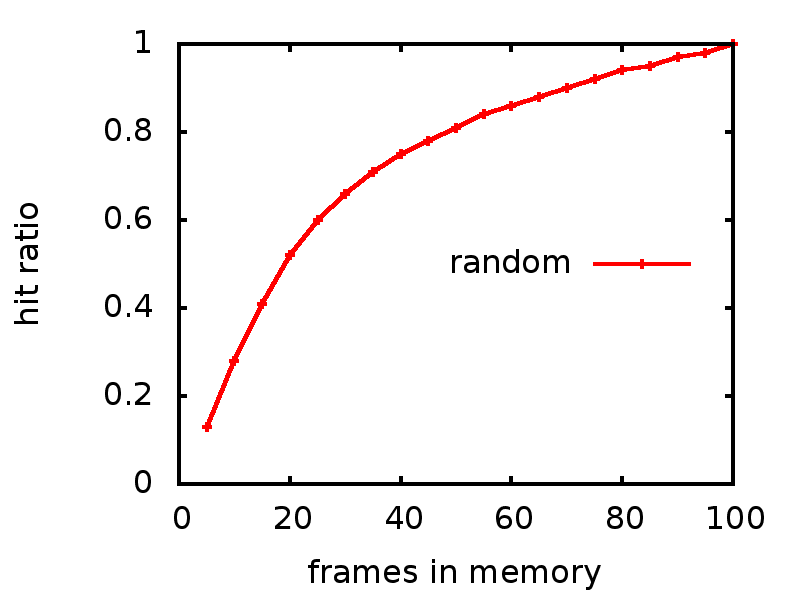
\includegraphics[scale=0.4]{random.png}
  \caption{The random data in a nice graph}.
  \label{fig:random}
\end{figure}
   
The figure ~\ref{fig:random} includes the graph in this document that
is prepared using \LaTeX. If you have not learned how to use \LaTeX
it's high time to do so. It's a bit of a learning curve but well worth
it once you start working on your thesis.

\section{The optimal solution}

In order to estimate how well our random solution works we implement
an optimal solution, even though we know that the optimal solution is
not something that we will be able to use in practice. The optimal
solution will throw out the page that will not be used for the longest
period in time. We can determine this since we have the complete
sequence of requests (something that we would of course not have in a
real situation.

The optimal solution is quite easy to implement but our implementation
will not be particularly efficient. When it is time to evict a page we
will simply go through all pages in memory and check how far down the
sequence of references that it is found. The page with the highest
value is selected.

\begin{lstlisting}

	pte *evict;

	/* initial values */
	int sofar = 0;
	int candidate = pgs;
	
	for(int c = 0; c < pgs; c++) {
	  if(table[c].present == 1) {
	    /* the page is allocated */
	    int dist = 0;
	    while(seq[i+dist] != c && i+dist < refs) {
	      dist++;
	    }
	    if(dist > sofar) {
	      candidate = c;
	      sofar = dist;
	    }
	  }
	}
	evict = &table[candidate];

	evict->present = 0;
	entry->present = 1;

\end{lstlisting}

Make a copy of {\tt random.c} called {\tt optimal.c} and do the
following changes to the {\tt simulation()} procedure. 

It is quite fun challenge to find a more efficient algorithm to
implement the optimal solution. It is obvious that it is a waste of
time to calculate the distance of all pages every time we have a page
fault. We should be able to keep a list of all the pages in memory, ordered by
the next position in the sequence. It's a bit tricky to figure out how
to do it but the solution is quite simple once you get it right. The
reward is not so much that we will cut the time for our benchmark in
half but the satisfaction of figuring out how to do it. 

\subsection{how to proceed}

If we look at the data we see that there is certainly some room for
improvement. Even if the optimal policy does not give us a system
without page faults the reduced number of faults would result in a
dramatic increase in performance. If we can implement something that is
only half-way towards the optimal policy much would be gained.

\section{Least Recently Used}

We will first implement something that works quite well, the {\em
  least recently used policy}. The only problem with this policy is
that it is quite costly and it is important to understand why this is. 

\subsection{a list of the last referenced pages}

Let's keep a list of the last referenced pages, the ones that are in
memory. We will keep the list ordered and have the least recently used
page first in the list and the most recently referenced page last in
the list. When we reference a page that is in memory the page is also
in the list. We then move the page to the end of the list to keep the
list ordered. If the memory is full we simply evict the page that is
the first page in the list since this page is the least recently used.

We could create a new data structure to keep track of the list but we
will keep things simple and extend the page table entry to also keep a
{\em next} and {\em previous pointer}. These pointers are used if the
page is present in memory and thus linked in the list.

\begin{lstlisting}
typedef struct pte {
  int id;
  int present;
  struct pte *next;
  struct pte *prev;  
} pte;
\end{lstlisting}

In the simulation we keep track of the {\em first} and {\em last}
element of the list. Keeping track of the last element will allow us
to quickly add a new entry to the end of the list. Keeping the list
double linked allows us quickly unlink an entry.


We can change the {\tt simulate()} procedure and the structure would look something like follows:


\begin{lstlisting}
int simulate(int *seq, pte *table, int refs, int frames, int pgs) {

  int hits = 0;
  int allocated = 0;

  pte *first = NULL;
  pte *last = NULL;  
  
  for(int i = 0; i < refs; i++) {
    int next = seq[i];
    pte *entry = &table[next];

    if(entry->present == 1) {
      hits++;
        :
      /* unlink entry and place last */
        :
    } else {
      if(allocated < frames) {
	allocated++;

	entry->present = 1;
	entry->prev = last;
	entry->next = NULL;
          :
        /* place entry last */
          :
      } else {
	pte *evict;

	evict = first;
	first = evict->next;

	evict->present = 0;

	entry->present = 1;
	entry->prev = last;
	entry->next = NULL;

          :
        /* place entry last */
          :
      }
    }
  }
  return hits;
}
\end{lstlisting}

The errors you will encounter when you implement the procedure is the
corner cases. It's straight forward to unlink an entry if its in the
middle of a list but what happens if its the first item in the list?
What if it's the only entry in the list? You will get it right but do
use a pen and paper and make some drawings of how the pointers have
changed.

\subsection{much better but costly}

If you get the data from the LRU implementation you should see that it
is better than the random selection. It could be even better if the
sequence of references had shown more temporal locality. The problem
of the LRU algorithm is that it will cost you even if you don't have a
page fault. If you look at the implementation of the random algorithm
you will see that hardly anything is done when we have a page hit, we
increment a counter but this is only for our purposes of collecting
some statistics. Compare this with the LRU implementation where a
double linked list must be manipulated. 

We can not expect to reduce the number of page faults much more than
what we have with the LRU algorithm (apart from having good luck) but
our hope is to stay close to LRU as possible even if we reduce the
amount of work done when we have page hit.


\section{The clock algorithm}

The clock algorithm is a clever algorithm that could be explained
in terms of a list similar to the one used in the LRU algorithm. The
difference is that the list is not updated with each reference. It
becomes a simple FIFO queue of entries which does not help us very
much.

The trick is that we keep an extra flag in the page table entry that
keeps track of if the page has been referenced since it was last
cleared. If the page that we are about to evict has the reference flag
set it is placed last in the list so it is given a {\em second chance}. 

If we will frequently will move entries from the beginning of the list
to the end of the list we might as well let the entries form a ring
where wee keep track of where the list starts. This is why it is
called the clock algorithm.

\subsection{a single linked list}

It turns out that we will be fine with a single linked circular list.
We will not unlink a random entry but only the first entry in the
ring and this is much easier if the list is only single linked. 

\begin{lstlisting}
typedef struct pte {
  int id;
  int present;
  int referenced;
  struct pte *next;
} pte;
\end{lstlisting}

Our {\em clock handle} will point to the last entry in the circular
list so the entry which is a candidate for eviction will be one entry
ahead. The simulator now has the following structure.

\begin{lstlisting}
int simulate(int *seq, pte *table, int refs, int frms, int pgs) {

  int hits = 0;
  int allocated = 0;
  pte *last = NULL;
	
  for(int i = 0; i < refs; i++) {
    int next = seq[i];
    pte *entry = &table[next];

    if(entry->present == 1) {
      entry->referenced = 1;
      hits++;
    } else {
      if(allocated < frms) {
	allocated++;
	entry->present = 1;
            :
        /* place the entry last in the list */
            :
      } else {
	pte *cand = last->next;

	while(cand->referenced != 0 ) {
	  cand->referenced = 0;
	  last = cand;
	  cand = cand->next;
	}
	cand->present = 0;
	cand->referenced = 0;

	entry->present = 1;
	entry->referenced = 0;	  
            :
        /* place the entry last in the list */
            :
      }
    }
  }
  return hits;
}
\end{lstlisting}

As you see there are only one tricky case - where we are still
building the ring. We have to cover the corner case were there are no
entries in the ring and we're adding the first one. Apart from this
the implementation is quite simple. If you look at the figures
generated you will see that it sometimes even outperforms LRU (but
this is more based on luck). 

Take a look at the code - what do we need to do when we have a page
hit? As you see we are in pair with LRU but with a very limited
amount of extra work. If the updating of the page table can be done
in hardware the overhead is negligible.

\subsection{problems and extensions}

All though the clock algorithms works fine in our benchmark, reality
is often more complicated. What will happen if all of the pages are
referenced? We will of course traverse the ring and reset the
reference flags and then evict a page that was actually referenced
since the last page fault. If we would have a counter we would be able
to at least choose a page that had been referenced the least number of
times. A time stamp would be able to give us information on when the
page was last used etc.

Using only one bit to keep track of frequently and recently used pages
is of course an approximation. There are more advanced implementations
but the problem is that wee must keep the overhead for page hits to a
minimum. You can take some penalty when we have a page fault but we
do not want to examine all frames in memory to decide which one to
evict. 

What ever we do we need to remember that real life is more complicated
than benchmarks. If we lure ourselves into thinking that the benchmark
sequence is what real life sequences look like then we might optimize
our system for the benchmarks rather than reality. To improve the
implementation it might be more important to make the frequent case as
fast as possible rather than trying to avoid a page fault at all costs. 


\end{document}
